\documentclass[12pt]{graduate-design-manual}
\usepackage{graphicx}
\usepackage{listings}
\usepackage{algpseudocode}
\usepackage{xcolor}
\usepackage{tocloft}
\usepackage{natbib}
\usepackage{fancyhdr}
\captionsetup{font={small}}
\tikzset{every picture/.style={font=\fontsize{10.5pt}{12pt}\selectfont}}
\renewcommand{\normalsize}{\songti\Times\fontsize{14pt}{20pt}\selectfont}

\classid{SJ005-1}
\title{基于xxxx算法的系统设计}
\academy{计算机信息工程学院}
\field{软件工程}
\class{23软件x}
\id{20000000}
\author{张 三}
\Instructor{李 四}
\InstructorTitle{副教授}
\ReviewingTeacher{王五}
\ReviewingTeacherTitle{副教授}
\thedate{2025}{05}


\begin{document}
\makecover
% 中文摘要部分
\begin{cnabstract}{基于 xxxx 算法的系统设计}{关键词 1；关键词 2；关键词 3；关键词 4}
    摘要正文示例内容，摘要正文示例内容，摘要正文示例内容，摘要正文示例内容，摘要正文示例内容，摘要正文示例内容，摘要正文示例内容，摘要正文示例内容，摘要正文示例内容，摘要正文示例内容，摘要正文示例内容，摘要正文示例内容。

    摘要正文示例内容，摘要正文示例内容，摘要正文示例内容，摘要正文示例内容，摘要正文示例内容，摘要正文示例内容，摘要正文示例内容，摘要正文示例内容，摘要正文示例内容，摘要正文示例内容，摘要正文示例内容，摘要正文示例内容。
\end{cnabstract}
	
% 英文摘要部分
\begin{englishabstract}{System Design Based on xxxx Algorithm}{Key word 1; Key word 2; Key word 3; Key word 4}
    Sample content of abstract text, sample content of abstract text, sample content of abstract text, sample content of abstract text, sample content of abstract text, sample content of abstract text, sample content of abstract text, sample content of abstract text, sample content of abstract text, sample content of abstract text, sample content of abstract text, sample content of abstract text.

    Sample content of abstract text, sample content of abstract text, sample content of abstract text, sample content of abstract text, sample content of abstract text, sample content of abstract text, sample content of abstract text, sample content of abstract text, sample content of abstract text, sample content of abstract text, sample content of abstract text, sample content of abstract text.
\end{englishabstract}

\contents
\begin{preamble}

此文档为常州工学院计算机信息工程学院毕业设计说明书
\end{preamble}
\pagenumbering{arabic}
\mainbody
\section{毕业设计（论文）要求与流程}
\subsection{毕业设计（论文）目的和任务}
毕业设计（论文）是本科专业培养方案中最后一个教学环节，这个环节是对四年
学习的总结和提高，是全面培养学生综合素质与实践能力的主要手段，更是学生毕业
及学位资格认证的重要依据。整个毕业设计（论文）过程是理论和实际相结合，书本
知识与生产实践相结合，学生个体独立学习与培养团队协作精神相结合的过程，通过
毕业设计（论文）将大大提高学生的整体综合素质，为走向社会、走上工作岗位打下
坚实基础。

鼓励毕业设计与就业岗位结合，提倡双导师制（由企业导师提出课题，与校内导师共
同指导毕业设计） 。对于将要到企业就业的学生，建议学生选择项目设计、开发类课题，
注重技术应用；对考研学生，可参与到教师的科研项目中，从事研究型项目；鼓励学生针
对社会流行的手机应用程序、网络游戏程序的开发作为课题。
\subsection{毕业设计（论文）教学的基本要求}
\begin{enumerate}
\item 使学生掌握查阅本专业相关技术资料和工具书的方法；
    \item 有针对性地安排学生进行调研，阅读中外文献资料，翻译科技外文；
    \item 通过调研和文献检索，了解课题研究的内容在国内外地位和发展动态；
    \item 根据课题任务和内容，制定合理可行的工作计划，制定技术方案，并通过与其它方案比较加以论证；
    \item 毕业设计—工程应用软件类课题，应完成系统或多个模块的软件设计，并能正常运行；
    \item 毕业设计—工程应用控制类课题，应完成系统或某几个模块的软硬件设计，并有实物，且能正常运行；
    \item 毕业论文—属于专题研究类课题，题目新颖且具有探索性，属于学科前沿，偏重于理论研究；
    \item 制定系统或模块的测试或调试方法，并对测试数据作出分析和评价；
    \item 通过实际工作的训练，培养学生分析和解决实际问题的能力和独立工作的能力；
    \item 使学生在思想作风、工作态度、组织纪律和团结协作等方面受到良好的训练，着力培养创新应用型人才的综合素质。	
\end{enumerate}
\subsection{毕业设计（论文）工作流程及要求}
毕业设计（论文）工作流程原则上按以下几个步骤进行：

\begin{enumerate}
    \item 选题：确定毕业设计（论文）课题及指导教师，课题类型分为“毕业设计”或“毕业论文”二种类型。
    \item 任务书：指导教师给学生下达毕业设计（论文）任务书，明确毕业设计（论文）课题和必须完成的任务。
    \item 开题报告：深入企事业、实验室实际现场，了解课题的来源及现状，通过调研采集数据，作出需求分析，确定课题实施方案，制定技术路线，在此基础上书写开题报告。开题报告字数不少于 3000 字，从以下八个方面写：1.课题来源及现状，2.设计要求，3.工作内容，4.设计方案，5.技术路线，6.预期目标，7.时间安排，8.参考文献。开题报告一律以文本的形式（不要用表格形式）填入系统框内，必要的图或表可采用附件形式单独提交并注明图号。
    \item 外文翻译：对指导教师下达的外文资料，进行阅读并翻译；外文的内容应结合毕业设计（论文）课题，选择与课题相关的专业外文资料，翻译工作量不少于 15000 个印刷符号（例如：Computer 是 8 个印刷符号）。提交时译文（在译文前加上外文翻译封面）和原文均要提交。
    \item 毕业设计过程检查：提交周进展记录、初期检查、中期检查、末期检查。
    \item 毕业设计说明书（论文）：毕业设计说明书（论文）的内容基本上按开题报告上的框架来书写，各部分的内容要充实、具体，对自己设计的部分，应当作为重点来写，包括系统的软、硬件设计，调试、现场测试，最后进行的总结。相关数据、表格、程序流程等要有分析、有说服力，大量的源程序清单、数据字典和数据库表建议作为附录。正文字数不少于 38000 个中文字符。
    \item 毕业设计说明书（论文）相似度检测：学生在提交毕业设计说明书（毕业论文）正稿前，必须进行相似度检测，原则上文字复制比不高于 20\%，总评成绩为优秀的毕业设计（论文）文字复制比一般不能高于 15\%。
    \item 毕业设计说明书（论文）评阅：毕业设计说明书（毕业论文）正稿通过相似度检测之后，指导教师、评阅教师分别评阅毕业设计说明书（论文），并写出评阅意见。
    \item 毕业设计（论文）答辩：主要流程：1.答辩学生按指定顺序进入答辩现场；2.答辩小组组长宣读学生毕业设计（论文）课题及要求；3.答辩学生用事先准备好的 PowerPoint 进行汇报、介绍；4.答辩小组成员查看相关资料；5.答辩小组成员进行提问及回答；6.答辩要有记录；7.学生退场，评定成绩；98.填写相关表格。
    \item 以上各环节的文档必须在毕业设计（论文）智能管理系统中在规定的日期前进行提交与审核，以加强毕业设计（论文）各环节的进程管理与质量监控。（http://bysj.czu.cn）
\end{enumerate}

\subsection{毕业设计（论文）操作流程}
毕业设计采用“常州工学院毕业设计（论文）智能管理系统” ，操程如下图\ref{fig:liuchengtu}所示。

\begin{figure}[H]
    \centering
    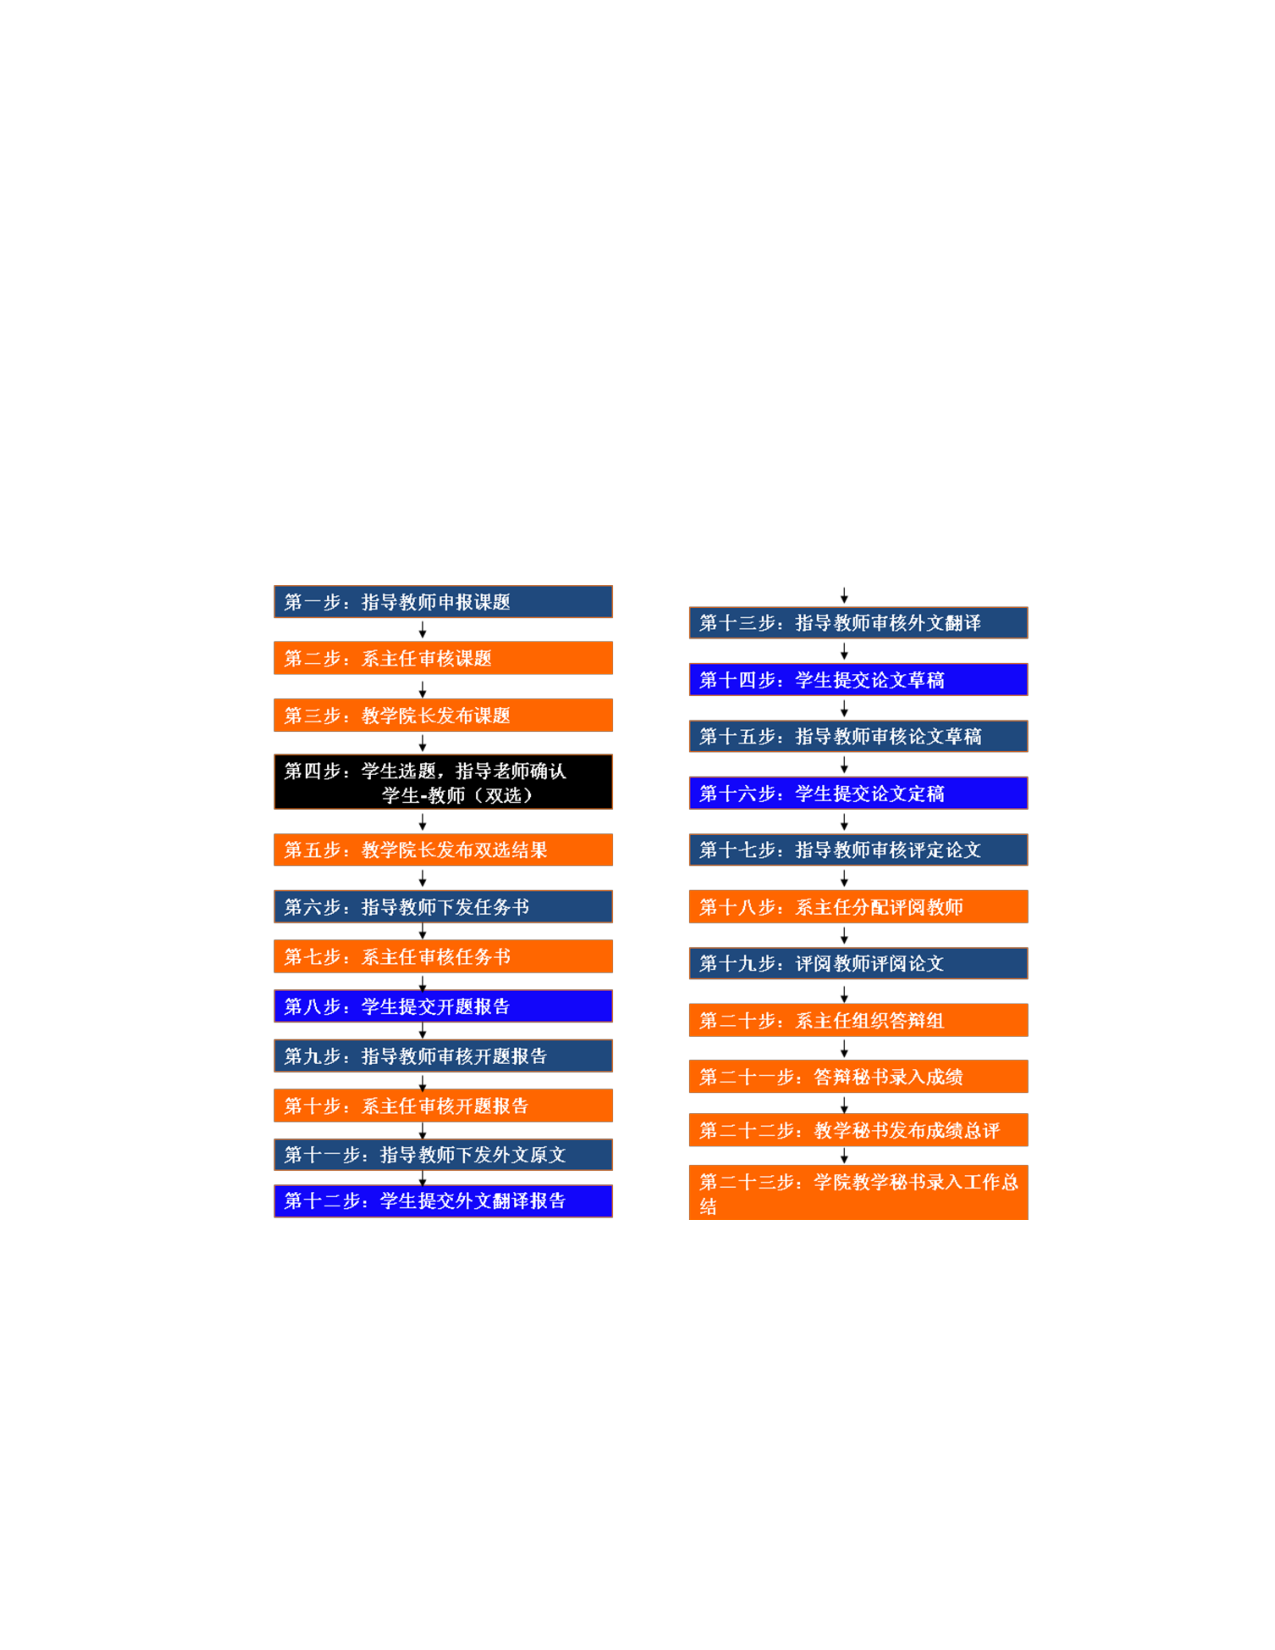
\includegraphics[width=0.8\textwidth]{figures/流程图.pdf}
    \caption{毕业设计（论文）操作流程}
    \label{fig:liuchengtu}
\end{figure}
\subsection{毕业设计（论文）成绩评定}
\begin{enumerate}
\item 使学生掌握查阅本专业相关技术资料和工具书的方法；
    \item 毕业设计（论文）综合成绩由指导教师评定成绩、评阅教师评定成绩和答辩成
绩三部分构成。各部分成绩评定独立进行，并按“毕业设计（论文）评分表指标”按
百分制打分。各部分成绩评定不受学生其它课程成绩的影响，主要是全面评价学生在
毕业设计（论文）全过程的学习、工作态度表、完成任务情况、选题的难易程度、毕
业设计说明书（论文）的内容与质量及研究成果。
    \item 答辩全部结束后由答辩小组对学生毕业设计（论文）成绩进行综合评定。综合
成绩评定根据指导教师的评定成绩、评阅教师评定成绩和答辩成绩，分别按学院规定
的权重系数求得（综合成绩=指导教师 30\%+评阅教师 20\%+答辩 50\%）。
\end{enumerate}

毕业设计（论文）综合成绩最终采用五级分制，即优秀、良好、中等、及格、不
及格。
\subsection{关于毕业设计（论文）重修}
毕业设计（论文）不及格者，可按学校规定，在下一学期的开学初到所在二级学
院办理返校重修申请，经二级学院教学院长审批同意后，由二级学院指定专业教师进
行指导。毕业设计重修时间的具体规定为：每年 12 月到下一年的 6 月，并严格按照
重修当年届（即下一届）的毕业设计指导书要求进行，采用“毕业设计智能管理系统”
全过程管理和监控，统一参加下一届的毕业设计答辩。
\subsection{取消毕业设计答辩资格}
存在下列情况之一的毕业设计学生，取消毕业设计答辩资格，成绩不予承认：1.
毕业设计材料不全或不符合要求的；2.毕业设计材料经指导教师审阅、或经评阅教师
评阅、或经二级学院审阅后，未达到参与答辩要求的；3.毕业设计说明书（论文）经
“中国知网”大学生论文检测系统检测后，总相似度大于 20\%；4.未参加二级学院统
一安排毕业设计答辩的；5.毕业设计存在弄虚作假行为的；6.毕业设计重修，但未办
理重修手续的。
\section{毕业设计说明书（论文）格式规范}
\subsection{用字、编辑、打印、顺序}
\subsubsection{版式、页眉、页边距及字体}
\paragraph{版式}
一律为 A4（210 ㎜×297 ㎜）
\paragraph{页眉}
页眉从摘要开始到最后，在每一页的最上方，用 5 号楷体，居中排列，页眉之下
划一条线，页眉内容根据课题类型选择“计算机信息工程学院毕业设计说明书”或“计
算机信息工程学院毕业论文”。
\paragraph{页边距}
页边距设置采取以下方式：上边距：2.5cm；下边距：2.1cm；左边距：2.1cm；右
边距：2.1cm；装订线：0.5cm；页眉：1.5cm；页脚：1.5cm；选择“不对称页边距”。
\paragraph{字间距和行间距}
字间距设置为：小四号宋体，加宽，0.2 磅。（在“字体”中设定）

行间距设置为：固定值 20 磅。（在“段录”中设定）
\subsubsection{用字、编辑与打印}
一律使用简化汉字，正文、摘要用字为小四号宋体。不得使用不合规定的简化字、

复合字、异体字或乱造汉字。如需要打印，一律采用 A4 双面打印。
编辑软件要求用 word 文字处理软件,.doc 文件。
\subsubsection{顺序}
毕业设计说明书（论文）顺序依次为封面、中文摘要、英文摘要、目录、前言、正
文、结论、致谢、参考文献、附录、在校学习期间获奖等评价情况。附录可按需列入。
\subsection{封面、中文摘要、英文摘要、目录的规范}
\paragraph{封面}
毕业设计说明书（论文）封面格式采用教务处统一格式，可在教务处网页“下载中
心”下载。

题目要做到确切、恰当、鲜明、简短，能概括整个文章最重要的内容。题目中所用
的词语应考虑到检索时可以提供特定的实用信息（如关键词）。题目字数要求在 25 字
以内。若题目语义未尽可用副题补充说明其特定内容。副题应处于从属地位，一般可
在题目的下一行用破折号“——
”引出。
\paragraph{中文摘要}
中文摘要不少于 300 字，摘要一般包括：文章的目的和重要性；采用的研究方法；
完成哪些工作；获得的主要结论。用句应精炼概括，并有文章的关键词 3－5 个。

摘要正文每行 37 个字（左右）；题目选三号宋体；正文选小四号宋体。

“关键词”三个字用宋体小四号加粗，关键词用小四号宋体。
摘要页无页码。

如图\ref{fig:cnabstract}所示:

\begin{figure}[H]
    \centering
    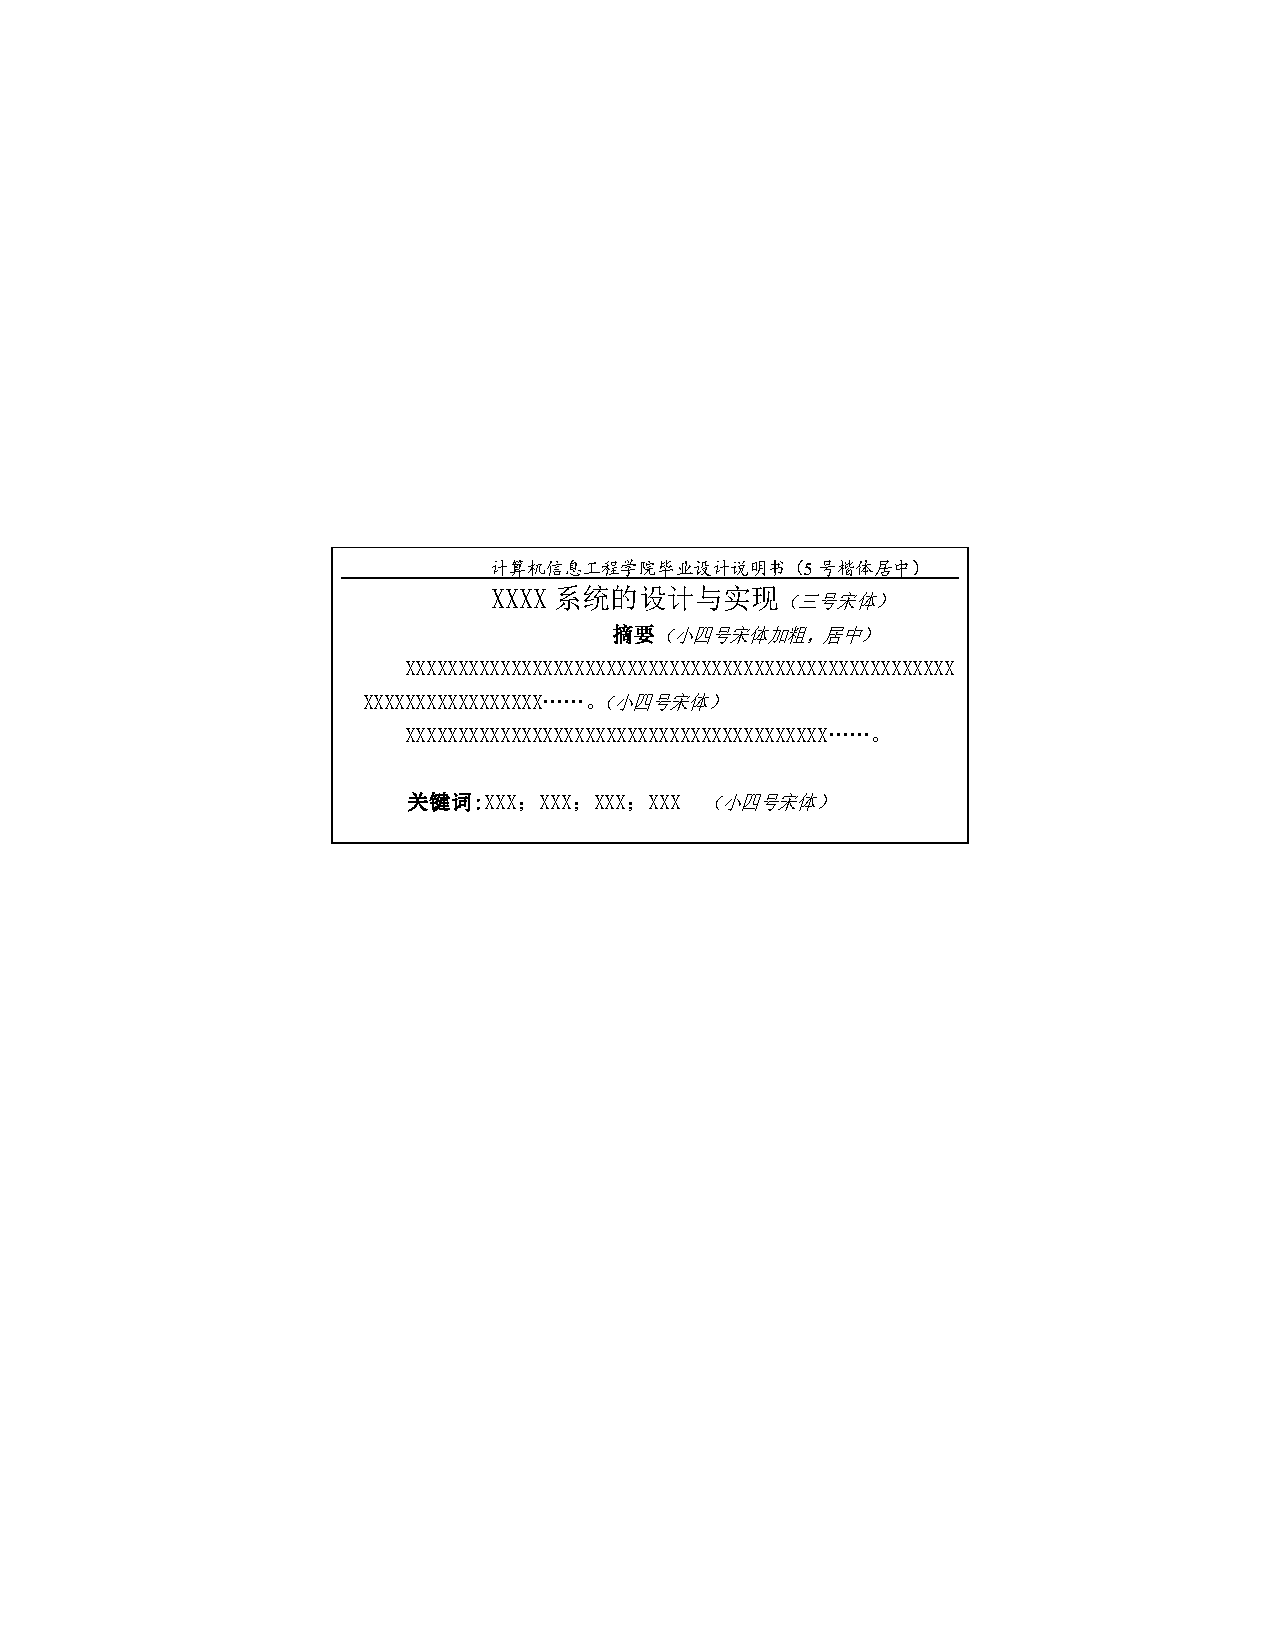
\includegraphics[width=0.8\textwidth]{figures/摘要.pdf} % 建议宽度设为页面的 0.8 倍
    \caption{中文摘要示例}
    \label{fig:cnabstract}
\end{figure}

\paragraph{英文摘要}
英文摘要是中文摘要的英文，不少于 1200 印刷字符。页眉写 Abstract，Times New
Roman 五号居中。

题目全部用大写字母，正文每行约 74 个字符。题目、Abstract 均选 Arial 四号加
粗，正文内容选 Times New Roman 小四号。

摘要页无页码。

英文摘要撰写要求如下：
\begin{enumerate}
    \item 用词应准确，使用本学科通用的词汇；
    \item 摘要中主语（作者）常常省略，因而一般使用被动语态，应使用正确的时态并要
注意主、谓的一致。必要的冠词不能省略；
\item “\textbf{Keywords}”一词用 Times New Roman 小四号加粗，关键词按相应专业的标准语
写出；
\item 中、英文摘要的内容须一致。
\end{enumerate}
\paragraph{目录}
\begin{enumerate}
\item 目录中章、节号均使用阿拉伯数字，目录层次到三级目录，参考格式如图\ref{fig:contents}所示，在 1.1 及 1.1.1 等层次中的“.”号用半角；
    \item 目录中应显示页码，页码右对齐，页码从正文开始直至全文结束，如图\ref{fig:contents}所示；
    \item 目录的页码另编，用“Ⅰ、Ⅱ、Ⅲ、Ⅳ、Ⅴ、Ⅵ、Ⅶ”小五号宋体；
\item 目录的页码在页下方居中排列，如图\ref{fig:contents}所示。
\end{enumerate}
\begin{figure}[H]
    \centering
    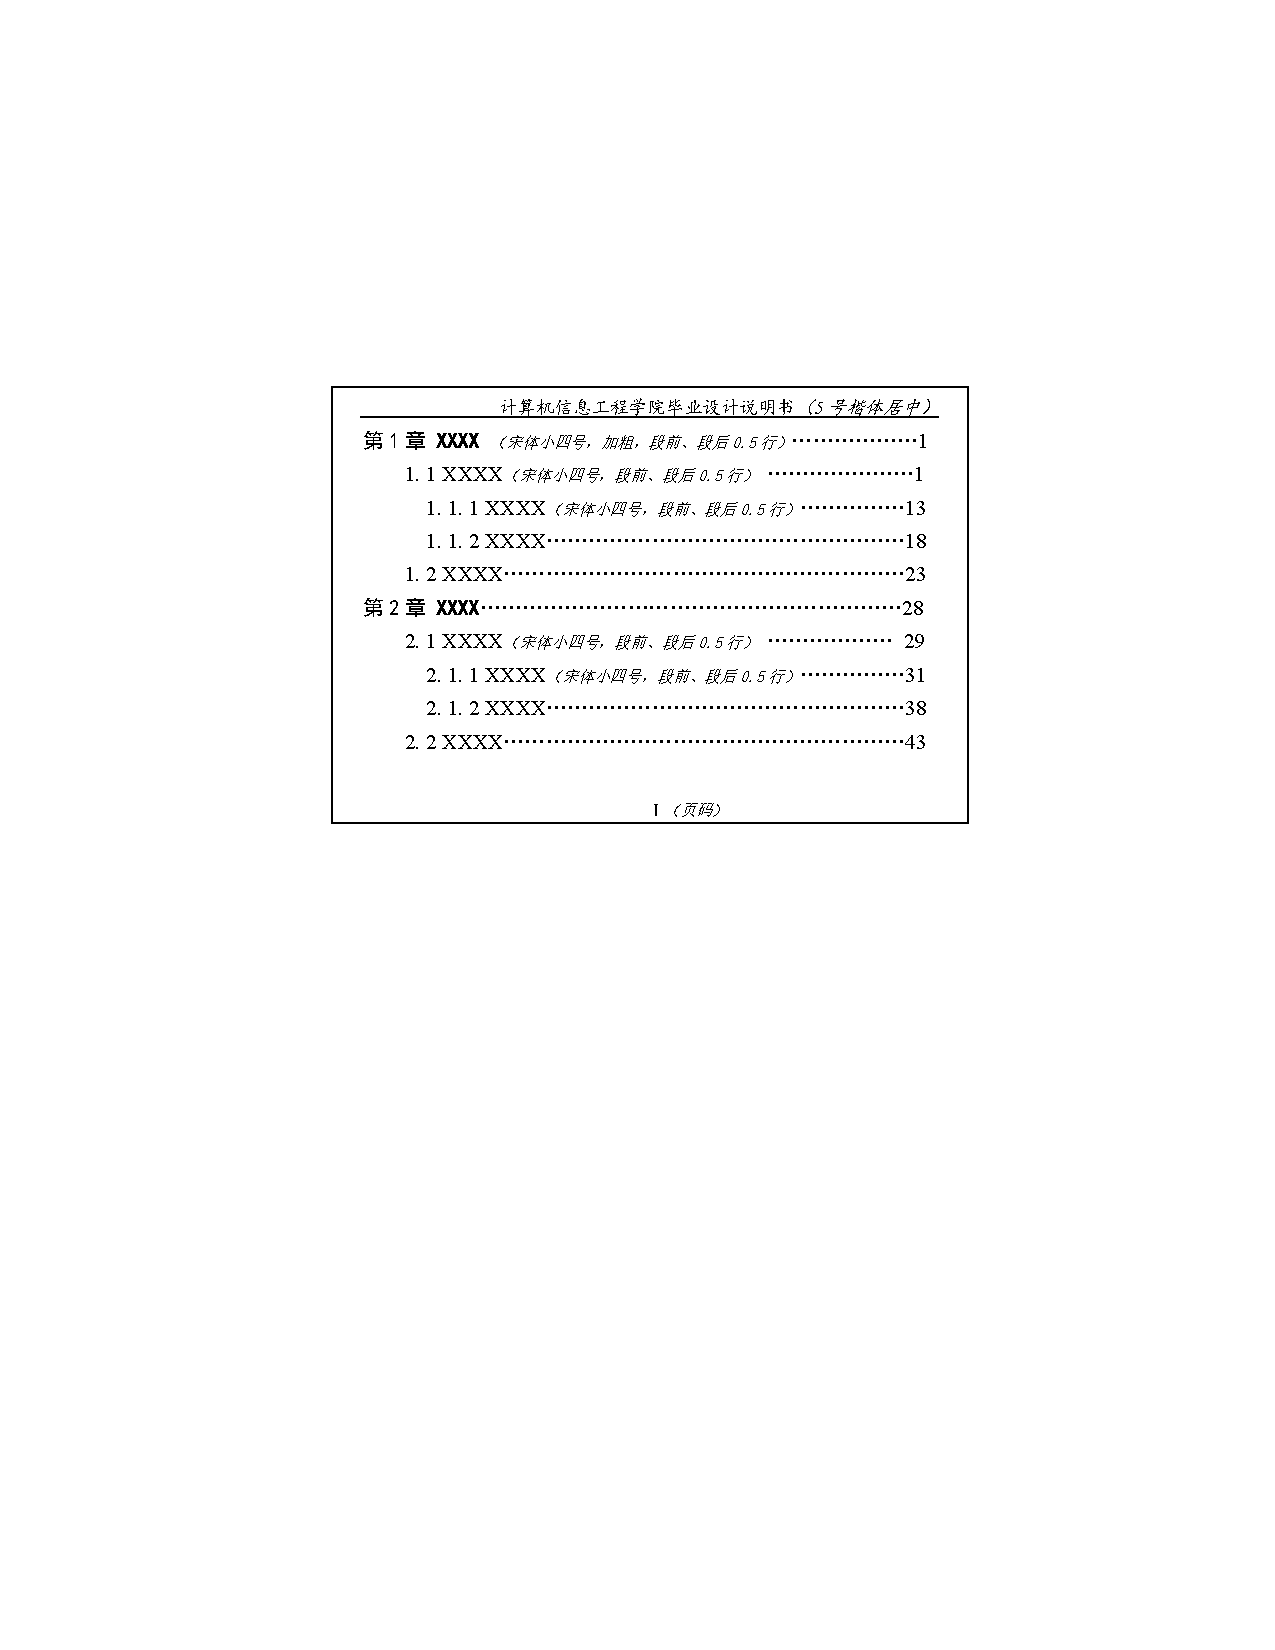
\includegraphics[width=0.8\textwidth]{figures/目录.pdf} % 建议宽度设为页面的 0.8 倍
    \caption{目录示例}
    \label{fig:contents}
\end{figure}
\paragraph{前言}
前言的内容可包括研究工作在国民经济中的实用价值和理论意义；本研究课题范围
内，国内外已有文献综述；理论依据和试验设备条件等。

前言页页码与目录页码连续，页码在页下方居中排列。

\subsection{正文的规范}
正文是一个逻辑严密、论述准确、结构合理、内容充实的整体，一般应包括研究
背景、主体研究内容及过程、结论等部分。作者可视具体研究内容分为若干章。全文
应与参考文献紧密结合，重点论述作者本人的独立研究工作和见解。文章不得模糊作
者与他人的工作界限，参考或引用了他人的学术成果或学术观点，必须给出参考文献，
严禁抄袭、占有他人的成果。正文页码从“正文、结论、致谢、参考文献、附录”一
直到全文结束，页下方居中排列，用“1、2、3、4、5、6……”数字。
\subsubsection{正文的层次格式}
正文的层次格式如下：
\vspace*{12pt}

\noindent\hspace{2em}{\fontsize{22pt}{20pt}\selectfont\heiti\bfseries 第 1 章 XXXX}（标题，二号粗黑体，居中；段前 1.5 行，段后 1 行；行距：固定值，20 磅）
XXXXXXXXXXXXXXXXXXXXXXXXXXXXX(内容，首行缩进 2 个字符，用小四号宋体；段前 0 行，段后 0 行；字间距设置为：加宽，0.2 磅；行间距设置为：固定值 20 磅)

\noindent\hspace{2em}{\fontsize{16pt}{20pt}\selectfont\heiti\bfseries 1.1 XXXXX}（标题，三号粗黑体，居左；段前 0.5 行，段后 0.5 行；行距：固定值，20 磅）
XXXXXXXXXXXXXXXXXXXXXXXXXXXXXX(内容用小四号宋体，首行缩进 2 字符；字间距设置为：加宽，0.2 磅；行间距设置为：固定值 20 磅)

\noindent\hspace{2em}{\fontsize{14pt}{20pt}\selectfont\heiti\bfseries 1.1.1 XXXX}（标题，四号粗黑体，居左；段前 0.5 行，段后 0.5 行；行距：固定值，20 磅）
XXXXXXXXXXXXXXXXXXXXXXXXXXXXXX（内容用小四号宋体，首行缩进 2 字符；字间距设置为：加宽，0.2 磅；行间距设置为：固定值 20 磅）

\noindent\hspace{2em}{\fontsize{12pt}{20pt}\selectfont\heiti\bfseries 1.XXXXX}（标题，小四号粗黑体，居左；段前 0.5 行，段后 0.5 行；行距：固定值，20 磅）

\noindent\hspace{2em}（1）XXXXXXXXXX（一句或一小段文字，以分号或句号结束；小四号宋体，居左；段前 0 行，段后 0 行；字间距设置为：加宽，0.2 磅；行距：固定值，20 磅）

例如图\ref{fig:mainbody}所示:

\begin{figure}[H]
    \centering
    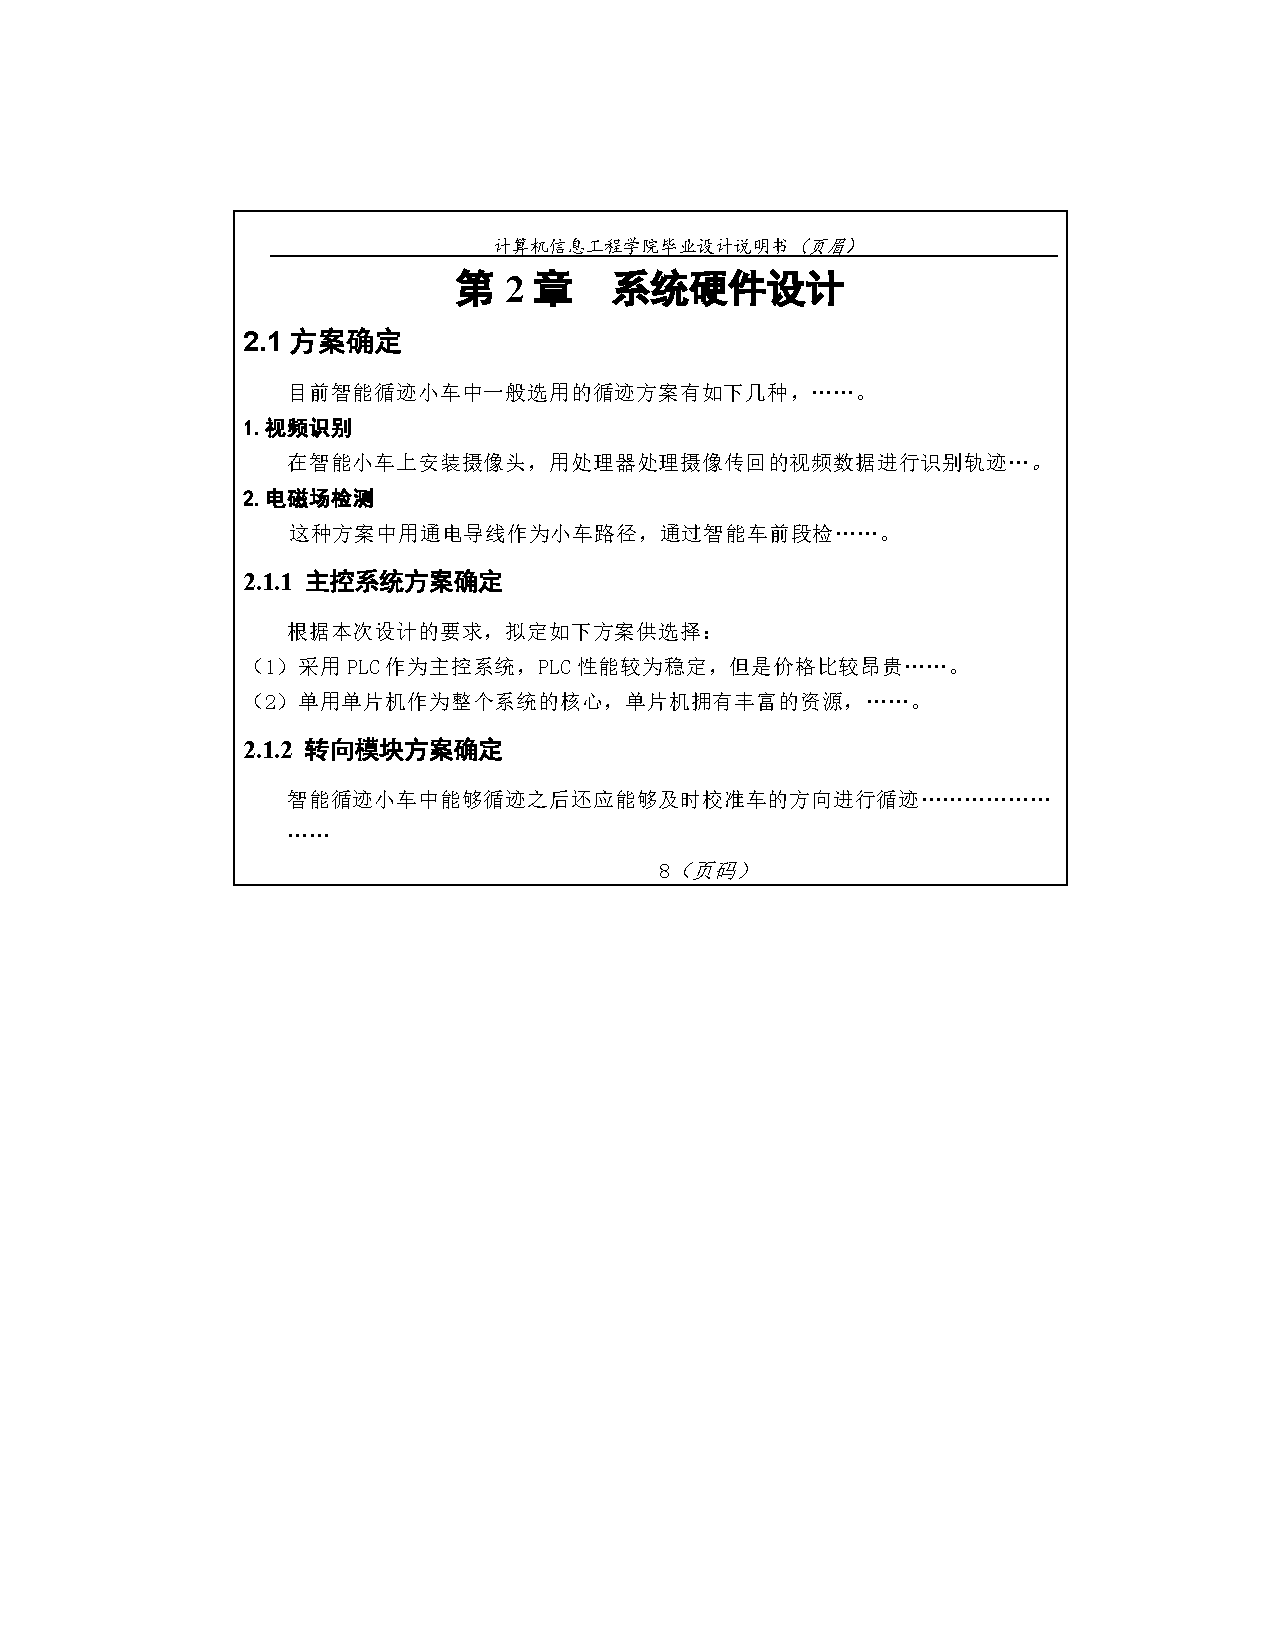
\includegraphics[width=0.8\textwidth]{figures/正文.pdf}
    \caption{正文示例}
    \label{fig:mainbody}
\end{figure}

\subsubsection{研究背景及意义}
研究背景是整个文章的基础，研究背景及意义的内容和要求为：
\begin{enumerate}
\item 清楚、严谨地论述国内外关于本课题研究领域的发展现状、水平及存在的问题；
\item 明确论述本研究的目的及意义；
\item 论述文章的研究思路和主要内容。
\end{enumerate}
\subsubsection{主体研究内容}
文章的主体一般包括：理论分析、计算方法、程序框图、程序段、实验装置和测
试方法、试验结果分析等。文章主体应力求准确、完整、清晰、通顺、实事求是、简
短精炼。

\subsubsection{结论}
结论要求简明扼要地概括文章所得出的若干重要结果和主要思想，包括理论分析、
模型建立及运算等结果，着重介绍作者本人的研究和成果及其在本学科或工程领域中
的地位和作用。结论要明确、精练、完整、准确。在结论中可以提出建议，进一步的
研究设想、仪器设备的改进、尚待解决的问题。

\subsubsection{插图、表格、公式、程序框图}
\paragraph{插图}
\begin{enumerate}[label=（\arabic*）]
    \item 所有插图必须有“图号”，图号按章编号，如第 1 章的第 1 张插图的图号为“图 1-1”；所有插图均需要有“图题”（即图的说明，用五号宋体），“图号”与“图题”间应空 1 个字距，在图的下方居中标出；
    
    例如：……采用运算放大器 LF353 设计的反相放大电路如图 \ref{fig:1-1}所示。
    
    \begin{figure}[htbp]
        \centering
        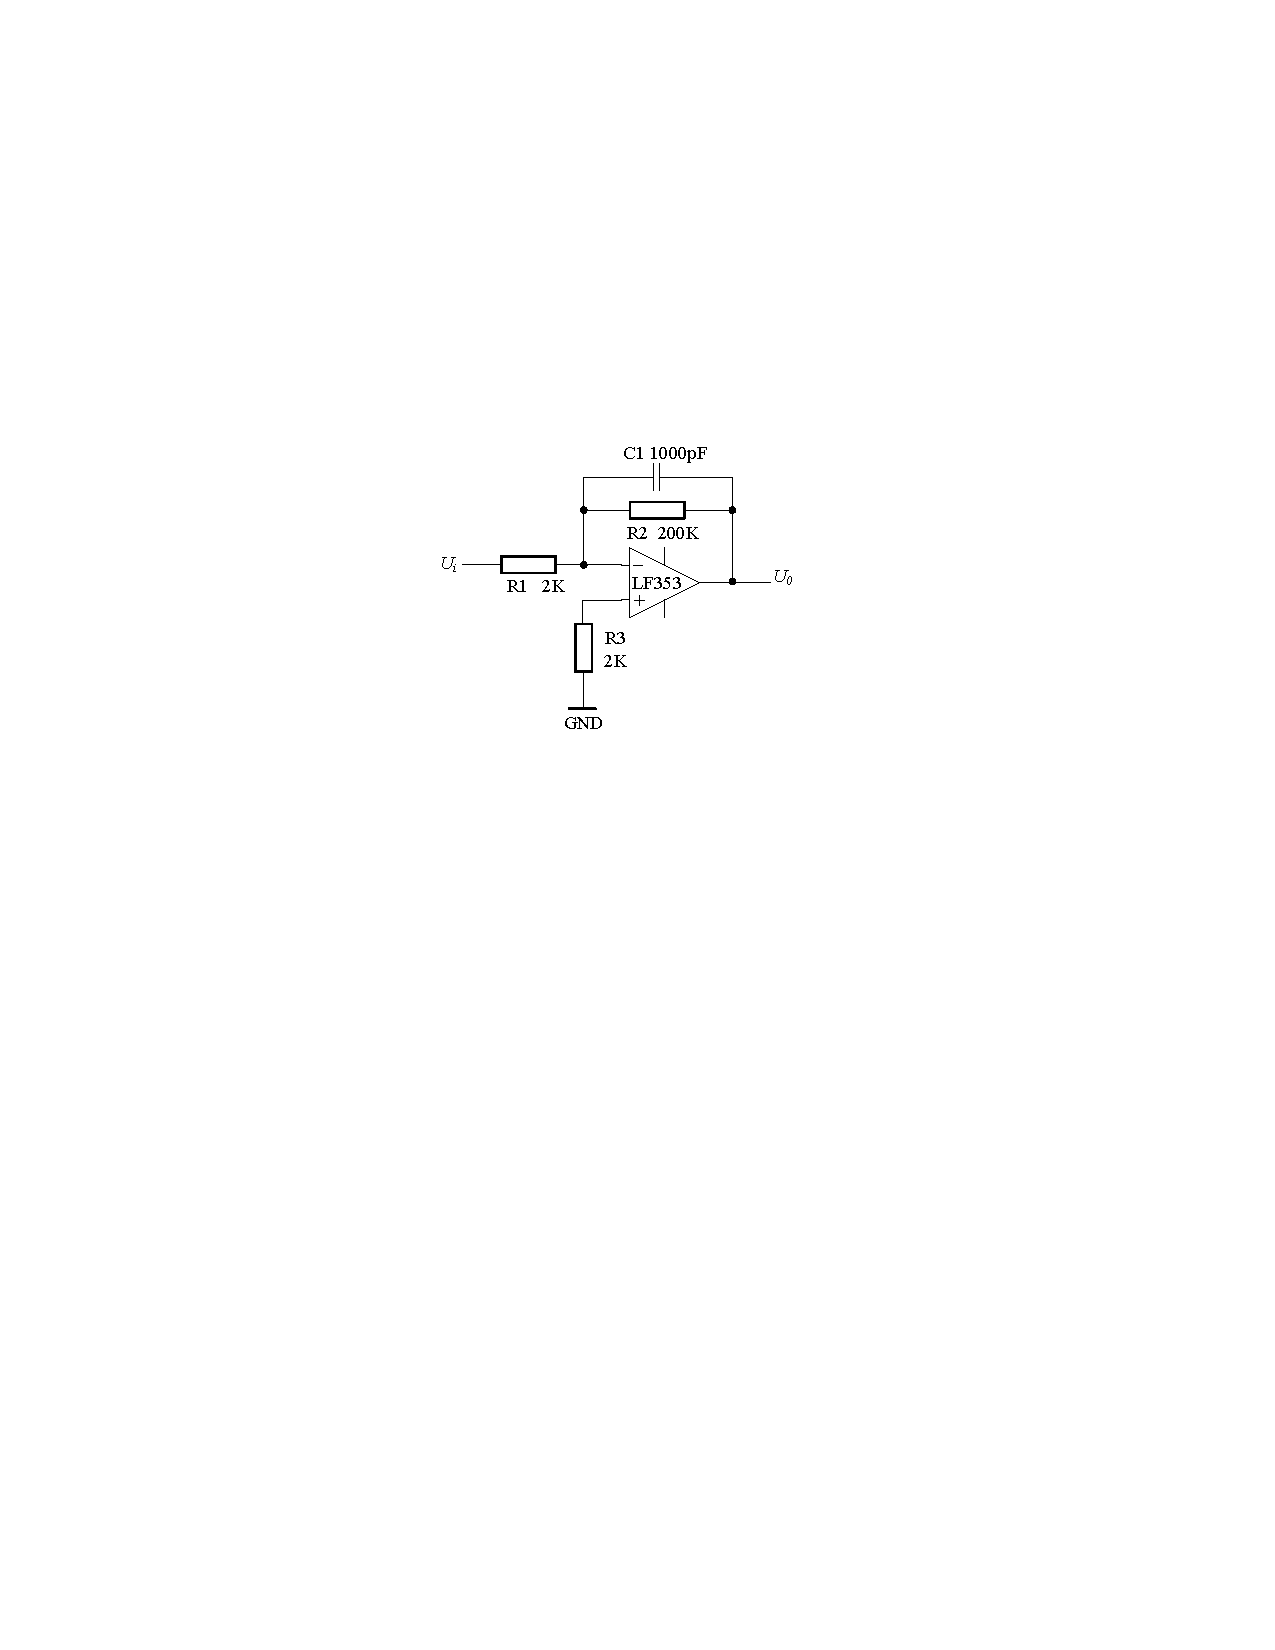
\includegraphics{figures/反相放大电路（5号宋体）}
        \caption{反相放大电路（5号宋体）}
        \label{fig:1-1}
    \end{figure}

    \item 一幅图如有若干幅分图，均应编分图号，用(a)，(b)，(c)……，按顺序编排；
    \item 插图须紧跟正文，特殊情况需延后的插图不应跨节；
    \item 图形符号及各种线型画法须按照现行的国家标准；
    \item 坐标图中坐标上须注明标度值，并标明坐标轴所表示的物理量名称及量纲，应均按国际标准（SI）标注；
    \item 图应具有“自明性”，即只看图、图题和图例，不阅读正文，就可理解图意；
    \item 图中用字为五号宋体。
\end{enumerate}
\paragraph{表格}
\begin{enumerate}
    \item 表格序号一律采用阿拉伯数字分章编号，如第 3 章第 1 个表的表序表示为“表 2-1”，并需有表题，表题应简明（用五号宋体）；
    \item 表格序号和表题间空 1 个字距，必须置于表格上方居中排列；
    
    \textit{例如：……测试数据如表\ref{tab:3-1} 所示。}
    
    \begin{table}[htbp]
        \centering
        \caption{测试数据表（5号宋体）}
        \label{tab:3-1}
        \begin{tabular}{|c|c|c|}
            \hline
            序号 & 延时（微秒） & 现象 \\ \hline
            1 & 40 & 不保护 \\ \hline
            2 & 30 & 不保护 \\ \hline
            3 & 25 & 不保护 \\ \hline
            4 & 23 & 不保护 \\ \hline
            5 & 20 & 保护 \\ \hline
        \end{tabular}
    \end{table}

    \item 表格的设计应紧跟正文。表格较大，不能在一页打印、需要转页排时，只需在续表上方居中注明“续表”，续表的表头应重复排出。若为大表或作为工具使用的表格，可作为附表在附录中给出；
    \item 表中各物理量及量纲均按国际标准（SI）及国家规定的法定符号和法定计量单位标注；
    \item 表格中的文字用五号宋体。
\end{enumerate}
\paragraph{公式}
\begin{enumerate}
    \item 公式均需有公式号；
    \item 公式号按章编排，如第 2 章的第 3 个公式序号为“（2.3）”；
    \item 公式中各物理量及量纲按国际标准（SI）及国家规定的法定符号和法定计量单位标注。禁止使用已废弃的符号和计量单位；
    \item 公式中用字、符号、字体要符合学科规范。
\end{enumerate}
\paragraph{程序框图}
\begin{enumerate}
    \item 程序框图也应有“图号”和“图题”，要求与“1. 插图”一样；
    \item 程序框图要符合规范，要有明确的流向（用箭头表示）；
    \item 程序框图所用字体：中文宋体五号，英文用 Times New Roman 体五号。
\end{enumerate}
\subsubsection{致谢}
\begin{enumerate}
	\item 致谢中主要感谢导师和对毕业设计（论文）工作直接有贡献及帮助的人士和单位。
谢辞应谦虚诚恳，实事求是。作者的家属及亲朋好友等与毕业设计（论文）无直接关
系的人员，一般不列入致谢范围；
	\item 致谢中还应感谢提供设计经费及实验装置企业的单位和个人。
\end{enumerate}
\subsubsection{参考文献}
    \begin{enumerate}
        \item 一律用 10.5pt 宋体（英文用 Times New Roman 体 10.5pt），字间距设置为：加宽 0.2 磅；行间距设置为：固定值 20 磅；
        \item 参考文献数量一般在 20 篇以上；一般选用实际查阅过并对文章有重要参考价值的文献；近 3 年内的学术文献不少于 10 篇；英文文献一般要 3 篇以上；
        \item 引用他人的学术观点或学术成果，必须列在参考文献中；
        \item 参考文献在整个文章中按出现先后依次列出，并在引用处右上角标注，标注符号为 \textsuperscript{【X】}；
        
        \textit{例如：“……发电效率可提高 25\%\textsuperscript{【1】}，……”}
        
        \item 参考文献著录格式示例：
    \end{enumerate}

    \begin{enumerate}[label={[\arabic*]}, itemsep=0pt, labelsep=0em]
        \item 主要责任者. 文献题目[M]. 出版地: 出版者, 出版年: 起止页码.
        \item 主要责任者. 文献题目[C]. 出版地: 出版者, 出版年: 起止页码.
        \item 析出文献主要责任者. 析出文献题名[C]. 原文献主要责任者. 原文献题名. 出版地: 出版者, 出版年: 析出文献起止页码.
        \item 主要责任者. 文献题目[D]. 出版地: 出版者, 出版年: 起止页码.
        \item 主要责任者. 文献题目[R]. 出版地: 出版者, 出版年: 起止页码.
        \item 主要责任者. 文献题名[J]. 刊名, 年, 卷(期): 起止页码.
        \item 主要责任者. 文献题名[N]. 报纸名, 出版日期(版次).
        \item 标准编号, 标准名称[S].
        \item 主要责任者. 电子文献题名[电子文献/载体类型标识]. 电子文献的出处或可获得地址, 发表或更新日期/引用日期.
        \item 主要责任者. 文献题名[Z]. 出版地: 出版者, 出版年.
        \item 专利所有者. 专利题名[P]. 专利国别: 专利号, 出版日期.
    \end{enumerate}

\subsubsection{附录的规范}
附录一律用 12pt 宋体（英文用 Times New Roman 体 12pt），字间距设置为：加宽 0.2 磅；行间距设置为：固定值 20 磅；内容包括：
    \begin{enumerate}
        \item 正文中过长的公式推导与证明过程可以在附录中依次给出；
        \item 与本文紧密相关的非作者自己的分析、证明及工具用表格等；
        \item 在正文中无法列出的实验数据；
        \item 正文中过大的程序框图；
        \item 正文中过大的电路图；
        \item 适量的原程序清单。
    \end{enumerate}
\section{一级标题}
\subsection{二级标题}
\subsubsection{三级标题}
这是正文。
\subsection{图片的引用}
在撰写毕业设计说明书时，插图是展示设计成果、程序流程及实验数据的重要手段。

对于普通的单张示意图，建议使用 [H] 选项以确保图片位置固定在正文描述之后。图应具有自明性，即读者仅通过阅读图、图题和图例，即可理解该图所表达的含义。坐标图中必须注明标度值，并标明物理量名称及量纲（按国际标准 SI 标注）。程序框图需符合规范，必须有明确的流向箭头。在实际写作中，建议先用 Visio 或 Figma 导出高清图片（推荐 PDF 或 PNG 格式），并预先调整好图片内的字号，以确保插入 LaTeX 后文字大小与正文五号字视觉一致。
\begin{figure}[H]
    \centering
    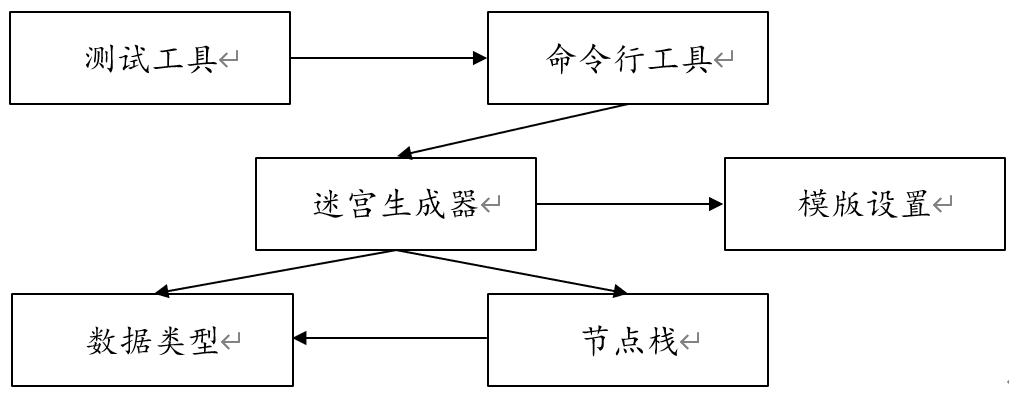
\includegraphics[width=0.8\textwidth]{figures/test.png}
    \caption{单张图片的标题名称}
    \label{fig:single_test}
\end{figure}

如果一幅图包含若干分图，必须编制分图号（如 (a)、(b)、(c)、(d)），并按顺序编排。
\begin{figure}[H]
    \centering
    % 第一行
    \begin{subfigure}{0.45\textwidth}
        \centering
        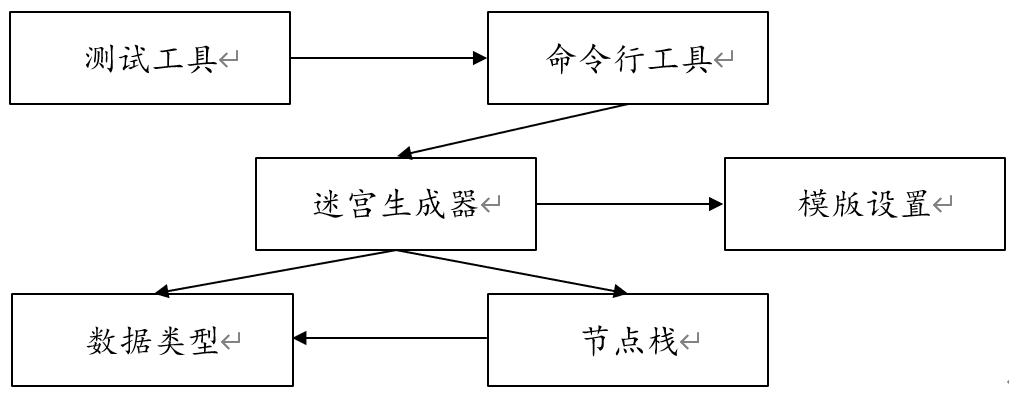
\includegraphics[width=\linewidth]{figures/test.png}
        \caption{分图 a 的说明}
    \end{subfigure}
    \hfill
    \begin{subfigure}{0.45\textwidth}
        \centering
        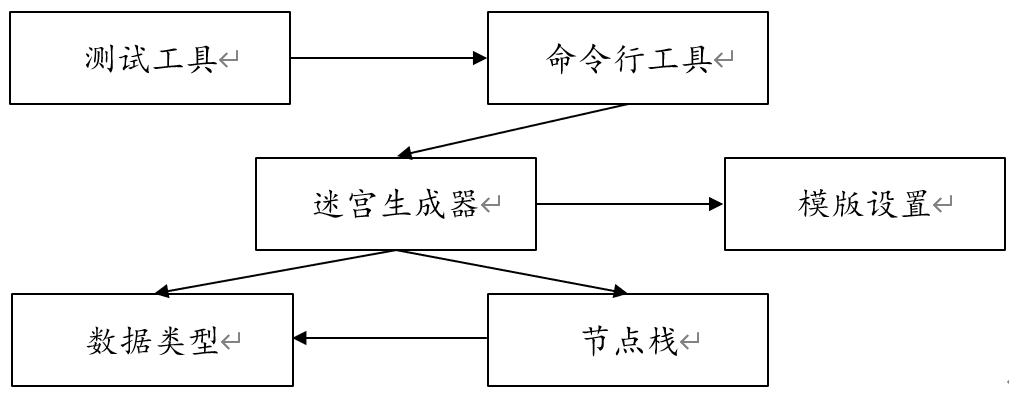
\includegraphics[width=\linewidth]{figures/test.png}
        \caption{分图 b 的说明}
    \end{subfigure}

    \vspace{1em}

    % 第二行
    \begin{subfigure}{0.45\textwidth}
        \centering
        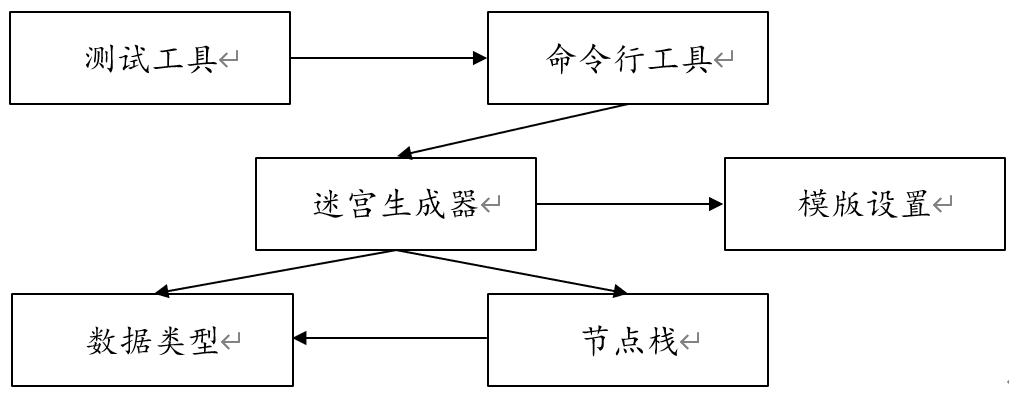
\includegraphics[width=\linewidth]{figures/test.png}
        \caption{分图 c 的说明}
    \end{subfigure}
    \hfill
    \begin{subfigure}{0.45\textwidth}
        \centering
        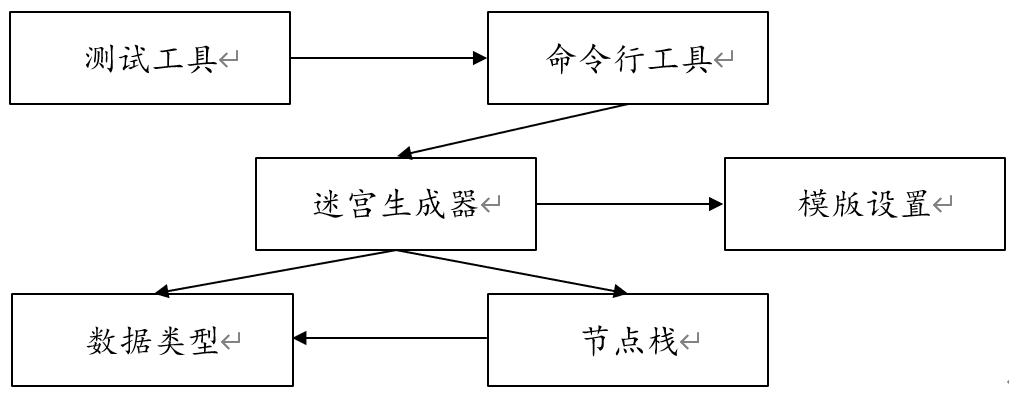
\includegraphics[width=\linewidth]{figures/test.png}
        \caption{分图 d 的说明}
    \end{subfigure}

    \caption{四宫格测试总图题}
    \label{fig:four_grid_test}
\end{figure}
\subsection{插入表格和公式}

本节主要介绍毕业设计说明书中表格与公式的编写规范及其在LaTeX中的实现方式。

\subsubsection{表格编写规范}

根据规范要求，表格的编排需遵循以下原则：

\textbf{表序与表题}：表格序号一律采用分章编号（如“表 3－1”），并配有简明的表题。

\textbf{位置与字号}：表序与表题应置于表格正上方居中，使用五号宋体。表序与表题之间应空 1 个字距。

\textbf{内容格式}：表内文字同样使用五号宋体。表格设计应紧跟正文，不宜跨节。

表格插入示例如下：
\begin{table}[H]
    \centering
    \caption{测试数据对比表}
    \label{tab:data_test}
    \begin{tabularx}{\textwidth}{YYYY}
        \toprule
        序号 & 实验项 & 测量值 & 备注说明 \\
        \midrule
        1 & 电压 (V) & 220.5 & 稳定状态 \\
        2 & 电流 (A) & 5.12 & 额定负载 \\
        3 & 功率 (W) & 1128.9 & 满载运行 \\
        \bottomrule
    \end{tabularx}
\end{table}
\subsubsection{公式编写规范}

公式的排版应符合学科规范，并使用法定计量单位：
\begin{itemize}
    \item \textbf{公式编号}：公式均需按章编排序号，序号需加圆括号并右对齐，如“（2.3）”。
    \item \textbf{量纲标注}：公式中各物理量及量纲必须按国际标准（SI）标注。
\end{itemize}

公式插入示例如下：

\begin{equation}
    P = \sqrt{3} U I \cos \phi
    \label{eq:power_calc}
\end{equation}

在正文中引用公式时，可以直接使用 \verb|\ref{eq:power_calc}|，系统会自动生成对应的编号。
\subsection{列表环境的使用}

在说明书正文中，为了使条目更加清晰，常使用无序列表和有序列表。本模板已通过 \texttt{enumitem} 宏包对列表间距进行了优化。

\subsubsection{无序列表（Itemize）}
无序列表适用于没有先后顺序的内容陈述。
\begin{itemize}
    \item \textbf{使用方法}：使用 \verb|\begin{itemize}| 环境。
    \item \textbf{格式要求}：列表内容应使用小四号宋体，行间距保持 20 磅。
\end{itemize}

\subsubsection{有序列表（Enumerate）}
有序列表适用于有步骤、等级或顺序要求的内容。
\begin{enumerate}
    \item 第一步：准备工作。
    \item 第二步：执行实验过程。
    \item 第三步：记录并分析数据。
\end{enumerate}

\subsection{代码清单与算法环境}

在软件工程及计算机相关专业的毕业设计中，核心算法的伪代码和关键源代码是展现系统实现细节的重要组成部分。

\subsubsection{源代码编写规范}

根据规范要求，代码清单的编排需遵循以下原则：
\begin{itemize}
    \item \textbf{格式要求}：代码中的中文应使用五号宋体，英文及数字使用五号 Times New Roman。本模板通过 \texttt{listings} 宏包已自动完成字体配置。
    \item \textbf{编号与标题}：代码清单通常参照插图规范处理，其图号按章编号（如“图 3－2”），图题应置于代码下方居中，使用五号宋体。
    \item \textbf{位置要求}：代码清单应紧跟正文描述，不应跨节排列。
\end{itemize}

代码插入示例如图 \ref{code:fastapi_impl} 所示：

\begin{listing}[H]
    \centering
    \begin{lstlisting}[language=Python]
from fastapi import FastAPI

app = FastAPI()

@app.get("/")
def read_root():
    # 这里的中文注释将自动渲染为五号宋体
    return {"message": "Hello, Changzhou Institute of Technology"}
    \end{lstlisting}
    \caption{FastAPI 后端接口实现示例}
    \label{code:fastapi_impl}
\end{listing}

\subsubsection{算法伪代码规范}

算法伪代码应具有明确的逻辑流向和规范的结构化表示：
\begin{itemize}
    \item \textbf{标题位置}：算法标题（如“算法 3－1”）应置于算法环境下方（参照插图规范），使用五号宋体。
    \item \textbf{字体要求}：算法中的描述性文字使用五号宋体，变量与公式使用五号 Times New Roman。
    \item \textbf{逻辑符号}：应使用标准的流程控制语句（如 If-Then-Else, While 等），并保持清晰的缩进结构。
\end{itemize}

算法示例如下所示：

\begin{algorithm}[H]
    \begin{algorithmic}[1]
        \Require 原始语音信号 $S$
        \Ensure 特征向量 $V$
        \State $S_{pre} \gets \text{Pre-process}(S)$ \Comment{调用预处理函数}
        \If{$S_{pre}$ is valid}
            \State $V \gets \text{CNN\_Extract}(S_{pre})$ \Comment{特征提取}
        \Else
            \State \Return \textbf{null}
        \EndIf
        \State \Return $V$
    \end{algorithmic}
    \caption{基于深度学习的方言特征提取算法}
    \label{alg:dialect_feat}
\end{algorithm}
\subsection{参考文献的编写}

参考文献是毕业设计说明书的重要组成部分，不仅反映了论文的科学依据和作者对他人研究成果的尊重，也为读者提供了进一步查阅相关资料的线索。

\subsubsection{编写要求}
\begin{itemize}
    \item \textbf{著录标准}：参考文献的著录应符合国家标准《信息与文献 参考文献著录规则》（GB/T 7714-2015）。
    \item \textbf{引用顺序}：正文中引用的文献应按出现先后顺序编码，并在引用处右上角用方括号注明序号（如 【1】）。
    \item \textbf{数量要求}：参考文献数量一般在 20 篇以上；一般选用实际查阅过并对文章有重要参考价值
的文献；近 3 年内的学术文献不少于 10 篇；英文文献一般要 3 篇以上。
    \item \textbf{实引对应}：文后的参考文献列表必须与正文中的引用一一对应，不得列入正文中未引用的文献。
\end{itemize}

\subsubsection{\LaTeX 实现}
模板推荐使用 Bib\TeX{} 技术进行文献管理。通过维护一个 \texttt{.bib} 格式的数据库文件，可以实现自动排序、自动生成编号以及格式化的文献列表。例如这里下面的引用：

随着深度学习的发展，文档图像处理技术取得了显著进步。
刘绍锴\cite{面向文档图像恢复的建模与学习方法研究}针对文档图像恢复问题提出了建模与学习的新方法。
在提高识别率方面，杜泽炎和任明武\cite{一种在低质量图像上提高字符识别率的深度学习框架}构建了一个专门针对低质量图像的识别框架。

此外，针对手写文本行的提取与识别，曾海霖\cite{复杂文档图像上手写文本行提取与识别方法的研究}进行了深入探讨。
在国际前沿技术中，Vision Transformer（ViT）在图像分类任务中表现优异\cite{TransformerInVision}，
其核心思想也广泛应用于图像识别领域\cite{DeepLearningForImageRecognition}。

% 如果需要同时引用多篇文献，可以用逗号隔开
许多学者对低质量文档的二值化及识别进行了研究\cite{超分辨率重建在低质量文本图像识别上的应用, 基于深度学习的低质量文档图像二值化算法研究}。
\begin{acknowledgement}
    在论文完成之际，我要衷心感谢我的指导老师...
    同时感谢常州工学院计算机信息工程学院提供的实验环境...
\end{acknowledgement}

\bibliographystyle{gbt7714-numerical}
\bibliography{report}
\appendixsection
\begin{appendixsection}
    \section{主要源代码}
    这里可以放置你的核心代码片段。由于模版已经配置了代码高亮环境，你可以直接使用：
    
    \begin{lstlisting}[language=Python, caption={核心算法实现}]
    def hello_czu():
        print("Hello, Changzhou Institute of Technology!")
    \end{lstlisting}

    \section{相关数据表格}
    如果有一些原始数据不方便放在正文中，可以放在这里。
    
    \section{调查问卷或其它支撑材料}
    补充说明材料。
\end{appendixsection}
\end{document}
